\section{Resultados}

\subsection{Verificación y alcance del núcleo de referencia}

La implementación del núcleo se contrastó con las ecuaciones y los
escenarios publicados por Eriksen. Esta verificación comprueba que el
código reproduce el modelo de referencia; no demuestra que el modelo
sea transferible sin reajuste a otros alimentos o sistemas de medición.

En Laganaro, la reproducción del \co{} individual presenta RMSE entre
$2{,}32$ y $3{,}54$ mg \co{}/d/larva. En Bekker, el intervalo es
$2{,}29$--$4{,}58$ mg \co{}/d/larva. Como esos escenarios ya
intervinieron en la parametrización original, se interpretan como
reproducción del modelo y no como validación independiente.

\subsection{Ajuste de calibración en los datos propios}

El núcleo original se aplicó sin lecho y sin reajuste a los ocho cierres
de gas. La tabla compara las observaciones con las predicciones del
modelo original y del modelo completo propuesto.

\begin{table}[H]
\centering
\small
\caption{Cierres propios y predicciones de la calibración completa;
no son predicciones fuera de muestra. Los valores precedidos por $\geq$
son cotas inferiores por saturación. Unidades: ppm/min.}
\begin{tabular}{l c r r r}
\toprule
Dieta & Día & Observado & Eriksen & Propuesto \\
\midrule
D1 & 6, R1 & $\geq670{,}56$ & $273{,}71$ & $469{,}38$ \\
D1 & 6, R2 & $\geq474{,}23$ & $273{,}71$ & $469{,}38$ \\
D1 & 8     & $\geq311{,}82$ & $315{,}69$ & $450{,}34$ \\
D1 & 10    & $285{,}57$     & $303{,}38$ & $290{,}47$ \\
D4 & 6     & $228{,}52$     & $247{,}59$ & $323{,}89$ \\
D4 & 8     & $\geq383{,}67$ & $308{,}53$ & $331{,}79$ \\
D4 & 10    & $104{,}11$     & $306{,}22$ & $144{,}13$ \\
D4 & 14    & $79{,}11$      & $236{,}72$ & $143{,}21$ \\
\bottomrule
\end{tabular}
\end{table}

\begin{table}[H]
\centering
\caption{RMSE censurado de calibración, calculado sobre los mismos
ocho cierres utilizados en el ajuste.}
\begin{tabular}{l r r r}
\toprule
Dieta & Eriksen & Propuesto & Reducción \\
 & (ppm/min) & (ppm/min) & del error \\
\midrule
D1 & $222{,}49$ & $100{,}65$ & $54{,}8$\,\% \\
D4 & $133{,}88$ & $66{,}14$ & $50{,}6$\,\% \\
Conjunto & $183{,}61$ & $85{,}16$ & $53{,}6$\,\% \\
\bottomrule
\end{tabular}
\end{table}

En la calibración completa, los cuatro cierres no saturados dan un RMSE
de $60{,}89$ ppm/min. La cobertura de las cuatro cotas saturadas es
$1/4$; por tanto, la reducción del RMSE no implica que todas las
predicciones superen los límites instrumentales observados.

El RMSE de los controles sin larvas es $7{,}82$ ppm/min para D1 y
$7{,}95$ ppm/min para D4. El módulo microbiano representa
satisfactoriamente esos controles, pero su contribución predicha al
tratamiento no explica por sí sola toda la diferencia entre modelos.

\subsection{Validación cruzada interna}

La capacidad predictiva se evaluó mediante siete pliegues agrupados por
dieta y día. Los dos cierres de D1 del día 6 se excluyeron conjuntamente.
En cada pliegue se retiraron también el control y las observaciones de
crecimiento del día evaluado, y se recalibraron las etapas 1 y 2. Se
compararon el modelo original sin reajuste (E0), el núcleo recalibrado sin
lecho (R), el lecho aditivo (A) y el modelo acoplado (C). Cada cierre de
tratamiento fue predicho una única vez fuera de la calibración.

\begin{table}[H]
\centering
\small
\caption{Desempeño fuera de calibración. El RMSE censurado incluye los
ocho cierres; el RMSE exacto utiliza únicamente los cuatro no saturados.}
\begin{tabular}{l r r r}
\toprule
Modelo & RMSE censurado & RMSE exactos & Cobertura saturados \\
 & (ppm/min) & (ppm/min) & (\%) \\
\midrule
E0 & $183{,}61$ & $128{,}81$ & $25$ \\
R  & $164{,}21$ & $151{,}34$ & $50$ \\
A  & $154{,}21$ & $155{,}44$ & $50$ \\
C  & $124{,}94$ & $137{,}20$ & $25$ \\
\bottomrule
\end{tabular}
\label{tab:validacion_cruzada}
\end{table}

El modelo C presentó el menor RMSE censurado conjunto. Frente a E0, la
reducción puntual fue $31{,}95$\,\%; frente a R y A fue $23{,}92$\,\% y
$18{,}98$\,\%, respectivamente. No obstante, en los cuatro cierres no
saturados, C obtuvo un error $6{,}51$\,\% mayor que E0. Tampoco aumentó la
cobertura de las cotas saturadas respecto de E0.

Las predicciones fuera de muestra muestran dos limitaciones localizadas.
C subestimó los dos cierres de D1 del día 6 y sobreestimó los puntos
posteriores al pico: el residuo fue $+146{,}81$ ppm/min en D1, día 10, y
$+200{,}07$ ppm/min en D4, día 14. Por tanto, la reducción conjunta no
implica una mejora uniforme a lo largo del experimento.

El bootstrap exploratorio por dieta y día, con 5000 remuestreos, produjo
para C un RMSE censurado mediano de $124{,}94$ ppm/min y un rango percentil
de $75{,}64$--$157{,}98$ ppm/min. La reducción frente a E0 presentó un
rango de $-82{,}19$\,\% a $52{,}46$\,\%, y fue positiva en $80{,}5$\,\% de
los remuestreos. Estos porcentajes describen el remuestreo de siete días;
no constituyen una probabilidad de superioridad ni un intervalo de
confianza de validación independiente.

\subsection{Sensibilidad e identificabilidad}

En la calibración canónica, el modelo estimó $154{,}90$ g de \co{} en D1 y
$87{,}96$ g en D4 durante 14 días. La suma aritmética de ambos escenarios
independientes fue $242{,}86$ g. La sensibilidad local se evaluó mediante
perturbaciones de $\pm10$\,\%; en los parámetros situados en una cota solo
se perturbó hacia el interior del dominio.

\begin{table}[H]
\centering
\small
\caption{Máximo efecto local por parámetro. El cambio del acumulado usa la
suma de los escenarios D1 y D4; el cambio del RMSE se expresa en ppm/min.}
\begin{tabular}{l r r}
\toprule
Parámetro & Cambio máximo del \co{} total & Cambio máximo del RMSE \\
\midrule
$a_{\max}$       & $5{,}49$\,\% & $13{,}72$ \\
$k_{\mathrm{ref,D1}}$ & $3{,}06$\,\% & $2{,}57$ \\
$\delta_{CS,D4}$ & $2{,}75$\,\% & $5{,}36$ \\
$f_{D4}$         & $1{,}70$\,\% & $7{,}24$ \\
$\delta_{CS,D1}$ & $1{,}41$\,\% & $1{,}11$ \\
$\rho$           & $0{,}18$\,\% & $0{,}26$ \\
$k_{\mathrm{ref,D4}}$ & $0{,}10$\,\% & $0{,}19$ \\
\bottomrule
\end{tabular}
\label{tab:sensibilidad_local}
\end{table}

El acumulado fue localmente poco sensible a $\rho$. El perfil de costo,
reoptimizando $a_{\max}$ y $f_{D4}$, confirmó que su límite superior no
queda bien identificado. En la malla evaluada, los perfiles con aumento de
costo $\leq1$\,\% correspondieron a $\rho$ entre $4{,}395$ y $15$ y
produjeron entre $237{,}06$ y $243{,}00$ g de \co{} en el escenario
conjunto. Esta región es una comparación exploratoria, no un intervalo de
confianza.

El parámetro $a_{\max}$ tuvo el mayor efecto local sobre el ajuste. Su
perfil favoreció valores próximos a la cota superior: el costo aumentó
$4{,}75$\,\% al fijar $a_{\max}=1{,}45$ y $11{,}14$\,\% al fijarlo en
$1{,}40$. En consecuencia, el valor calibrado se reporta como un óptimo en
frontera dentro del rango declarado, no como una estimación fisiológica
precisa y libre de restricciones.

\subsection{Por qué Eriksen no describe apropiadamente los datos propios}

El desempeño del modelo original combina tres limitaciones.

\paragraph{Ausencia de la fuente microbiana.}
El núcleo original produce únicamente \co{} larvario, mientras el
observable propio corresponde al total de cámara. Los controles confirman
que existe una señal sin larvas. No obstante, añadir una fuente aditiva
no basta para corregir toda la discrepancia.

\paragraph{Transferencia de parámetros fuera de su dominio.}
Los valores originales se aplicaron sin recalibrar a otro alimento,
otra densidad de larvas y otro sistema experimental. En D1, día 6, la
predicción original de $273{,}71$ ppm/min queda aproximadamente
$59$\,\% por debajo de la cota de $670{,}56$ ppm/min. En D4 ocurre lo
contrario al final del experimento: el modelo predice
$306{,}22$ ppm/min frente a $104{,}11$ ppm/min en el día 10 y
$236{,}72$ ppm/min frente a $79{,}11$ ppm/min en el día 14.

\paragraph{Ausencia de acople dinámico con el alimento.}
En el modelo original, $a_d=a_{\max}$ mientras no se active el límite de
desarrollo. El alimento no reduce progresivamente la asimilación a
medida que se consume. En cambio, el modelo propuesto utiliza
$f_dD_C/(K_D+D_C)$, lo que permite una disminución más temprana del
\co{} en D4 y una trayectoria diferente entre dietas.

El diagnóstico neto larvario del modelo propuesto todavía presenta un
RMSE conjunto de $108{,}15$ ppm/min. Por tanto, la mejora total no debe
interpretarse como una reconstrucción perfecta de la respiración
individual.

\subsection{Descomposición del \co{} predicho}

La contribución microbiana predicha en D1 aumenta desde $9{,}6$\,\% en
el día 6 hasta $13{,}5$\,\% en el día 8 y $27{,}9$\,\% en el día 10.
En D4 disminuye desde $8{,}0$\,\% y $4{,}6$\,\% en los días 6 y 8
hasta $0{,}7$\,\% y aproximadamente $0{,}02$\,\% en los días 10 y 14.

Estas diferencias muestran que el lecho tiene un papel dinámico y
dependiente de la dieta. Sin embargo, la partición tratamiento menos
control no siempre es físicamente interpretable: en D4, día 14, esa
diferencia observacional es $-28{,}9$ ppm/min. El resultado refuerza la
necesidad de modelar el sistema acoplado en lugar de asignar
directamente toda la diferencia a las larvas.

\begin{figure}[H]
\centering
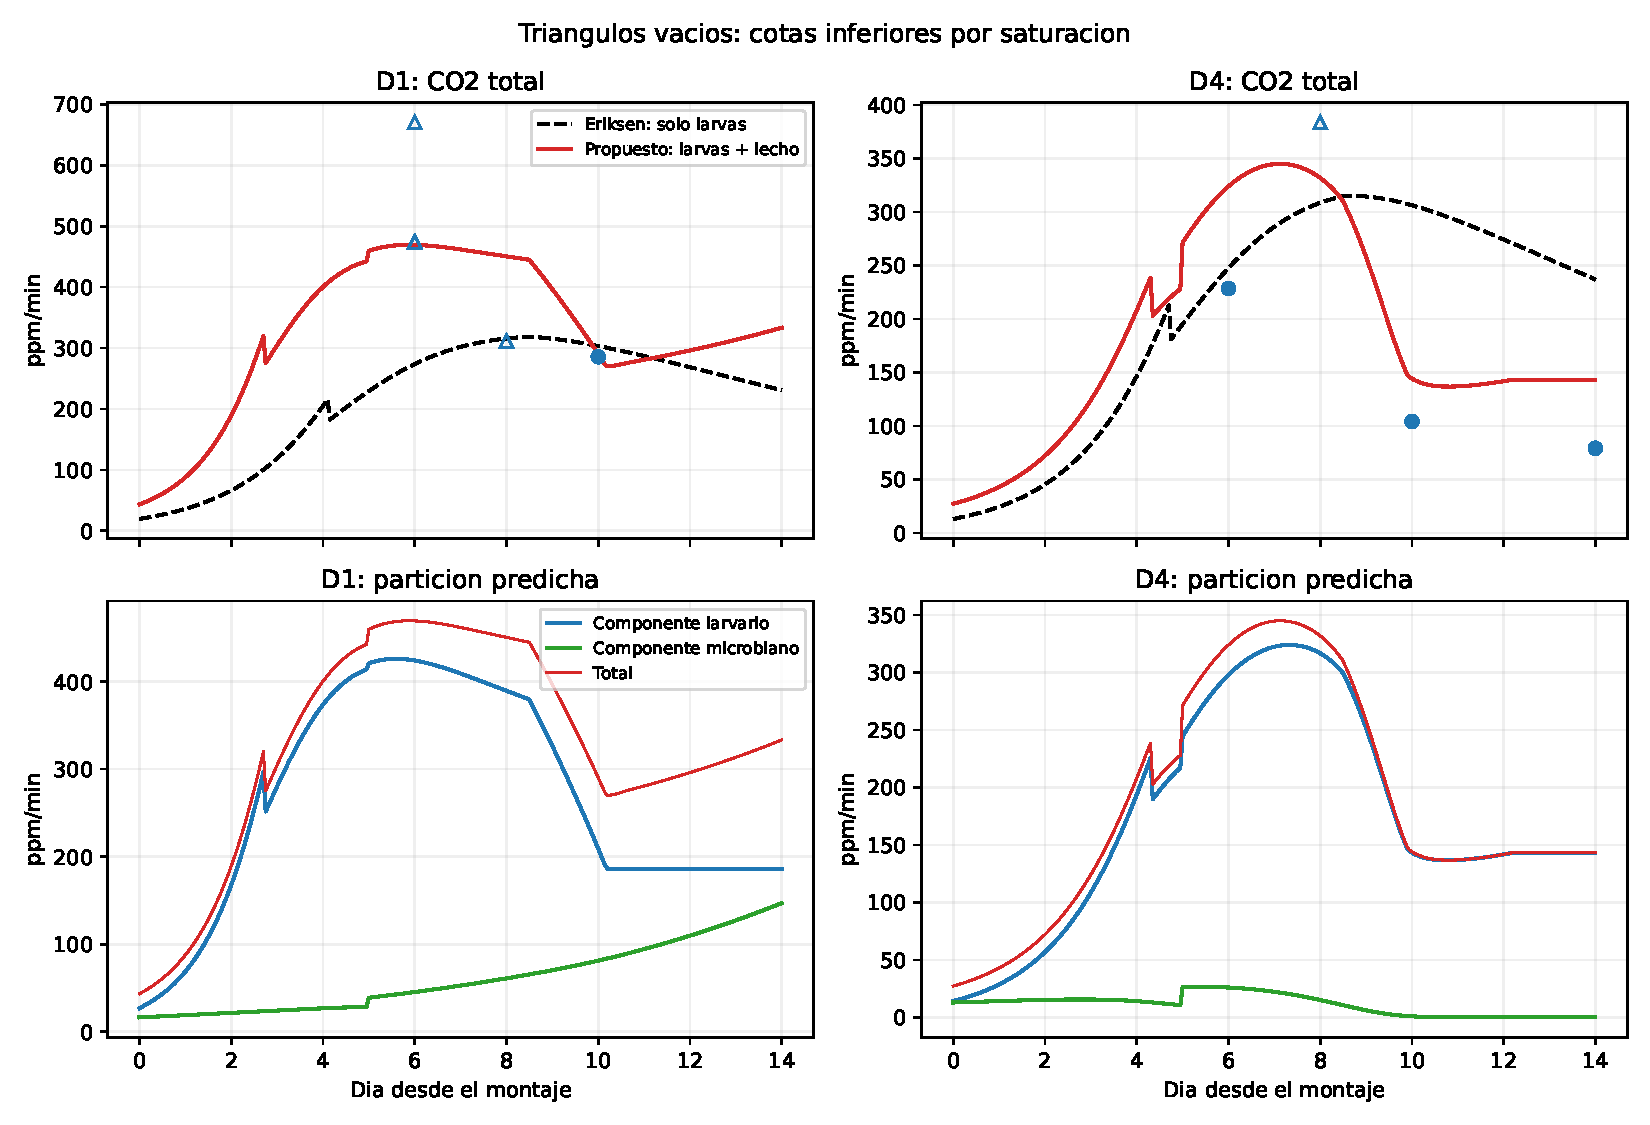
\includegraphics[width=\textwidth]{datos_propios_modelos.pdf}
\caption{Datos propios. Paneles superiores: Eriksen original y modelo
completo propuesto frente a los cierres observados. Paneles inferiores:
descomposición del modelo propuesto en componentes larvario y
microbiano. Los triángulos vacíos representan cotas inferiores por
saturación.}
\label{fig:datos_propios}
\end{figure}

\subsection{Transferencia externa}

\paragraph{Laganaro.}
Para la dieta sin lodos, el máximo específico observado es
$0{,}35$ d$^{-1}$ y el propuesto $0{,}42$ d$^{-1}$, con un error de
$+20$\,\%. Con 75\,\% de lodos, el observado aumenta a $0{,}64$ d$^{-1}$,
mientras el propuesto disminuye a $0{,}30$ d$^{-1}$, con un error
aproximado de $-52$\,\%. El factor $f_{D4}$ reduce disponibilidad, pero
no representa el aumento de costos metabólicos de una dieta de baja
calidad.

\paragraph{Bekker.}
El RMSE individual agrupado del modelo propuesto es
$1{,}50$ mg C/d/larva; por humedad, varía entre $1{,}19$ y
$1{,}76$ mg \co{}/d/larva. El intervalo correspondiente de Eriksen es
$2{,}29$--$4{,}58$ mg \co{}/d/larva. Sin embargo, el modelo propuesto
anticipa el pico individual entre $2{,}56$ y $7{,}50$ d, frente a
$0{,}67$--$2{,}59$ d en Eriksen.

El modelo propuesto reproduce algunos acumulados totales por
compensación de errores, pero no la partición de fuentes. Predice una
fracción microbiana aproximada de $66$--$67$\,\% en todas las humedades,
mientras la observada disminuye desde $78{,}1$\,\% hasta
$28{,}4$\,\%. El RMSE del total varía entre $0{,}49$ y
$1{,}80$ g C/d.

\paragraph{Ermolaev.}
En los días 2, 7 y 11, los flujos observados son $2{,}53$, $8{,}04$ y
$5{,}58$ mg/min. El modelo propuesto predice $4{,}69$, $9{,}04$ y
$4{,}98$ mg/min, con RMSE de $1{,}42$ mg/min, frente a
$1{,}83$ mg/min de Eriksen. No obstante, el acumulado propuesto es
$116{,}4$ g/kg FW, un $26$\,\% superior al observado de
$92{,}4$ g/kg FW, mientras Eriksen predice $75{,}8$ g/kg FW, un
$18$\,\% inferior. El pico propuesto ocurre en el día $5{,}1$, antes
del máximo observado alrededor del día 7.

\paragraph{Schøn.}
A $27{,}0$, $35{,}3$, $39{,}4$ y $41{,}9$ $^\circ$C, los totales
observados son $50$, $54{,}5$, $53$ y $24$ L/kg. El modelo propuesto
predice $81{,}6$, $90{,}3$, $98{,}2$ y $104{,}8$ L/kg, con errores de
$+63$\,\%, $+66$\,\%, $+85$\,\% y $+337$\,\%. El término $Q_{10}$
microbiano incrementa la emisión con la temperatura y no representa el
colapso observado a $41{,}9$ $^\circ$C.

\paragraph{Rossi.}
El modelo propuesto acumula $31{,}07$ g de \co{} total y
$11{,}05$ g en el control, con una diferencia neta de $20{,}02$ g.
Los valores netos observados son $5{,}55$, $32{,}38$ y $37{,}30$ g.
El RMSE neto disminuye desde $23{,}27$ g con Eriksen hasta
$14{,}84$ g con el propuesto, pero ninguno reproduce adecuadamente las
tres corridas. Además, el pico total propuesto ocurre en el día
$10{,}34$, frente a los días 5--7 observados.

\begin{figure}[H]
\centering
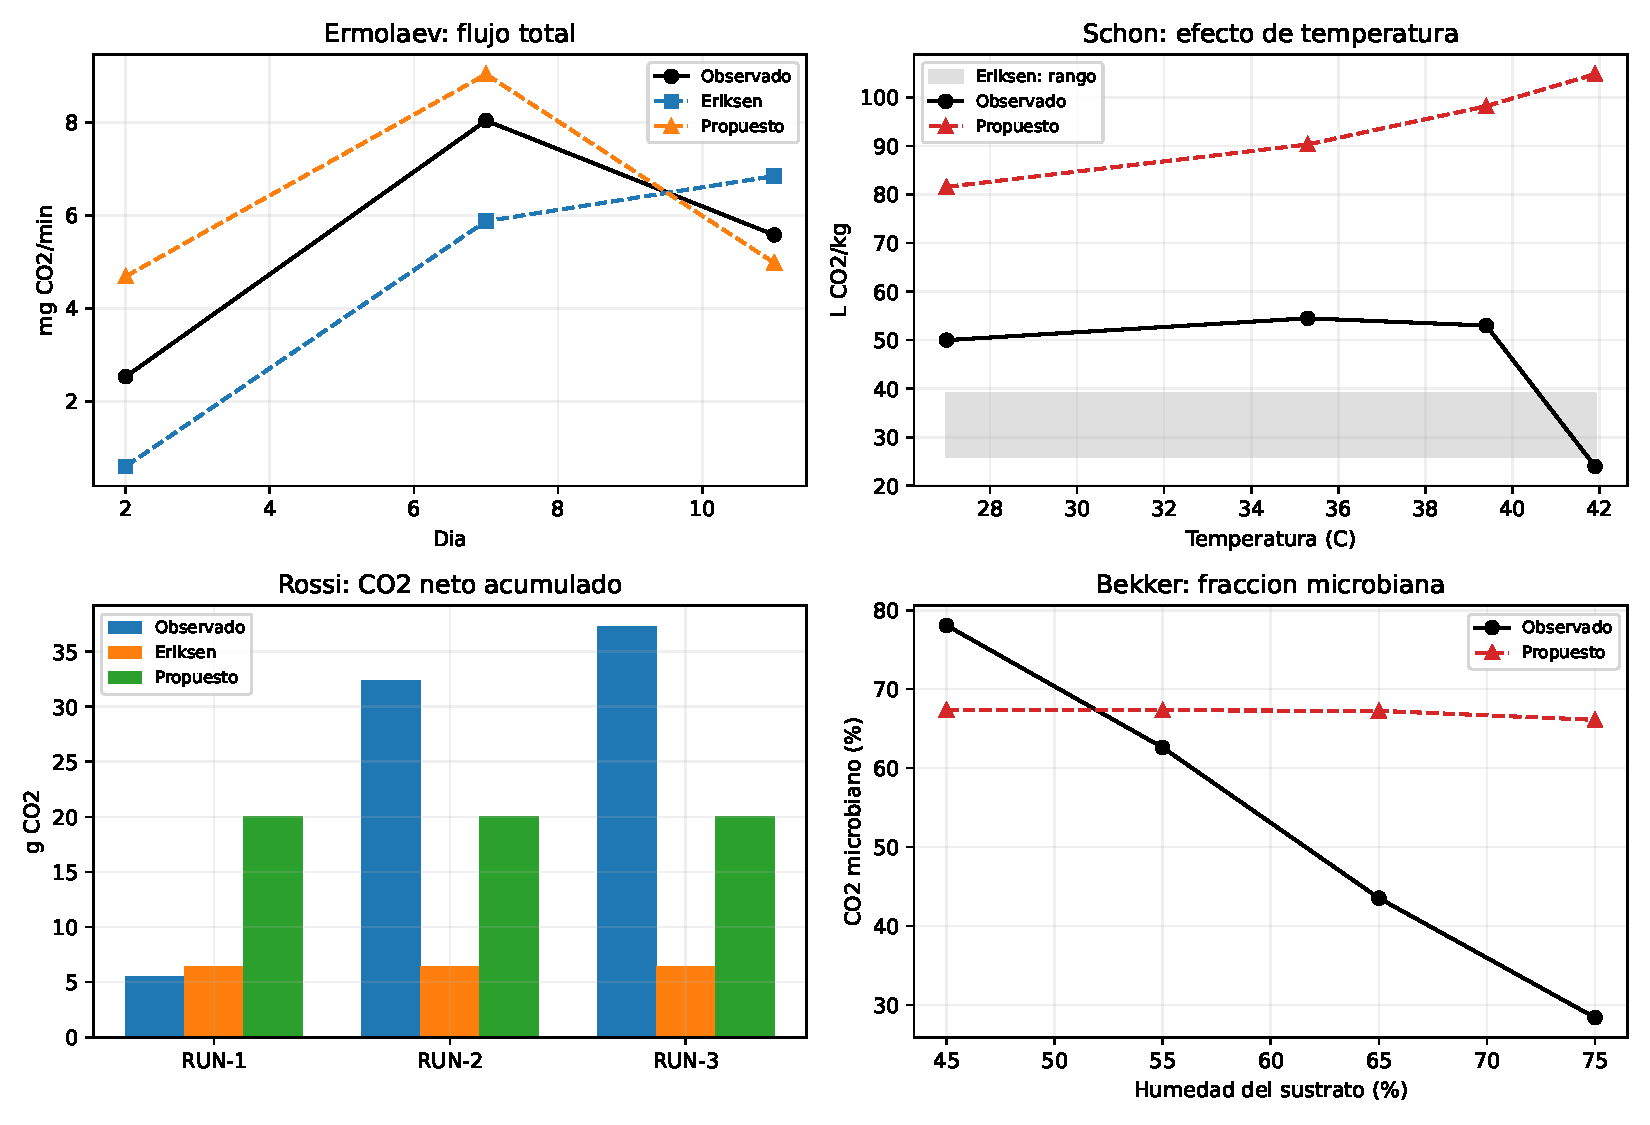
\includegraphics[width=\textwidth]{comparacion_externa.pdf}
\caption{Comparación externa de los observables publicados. Cada panel
conserva sus propias unidades y no debe interpretarse como una escala
común entre estudios.}
\label{fig:comparacion_externa}
\end{figure}

\begin{figure}[H]
\centering
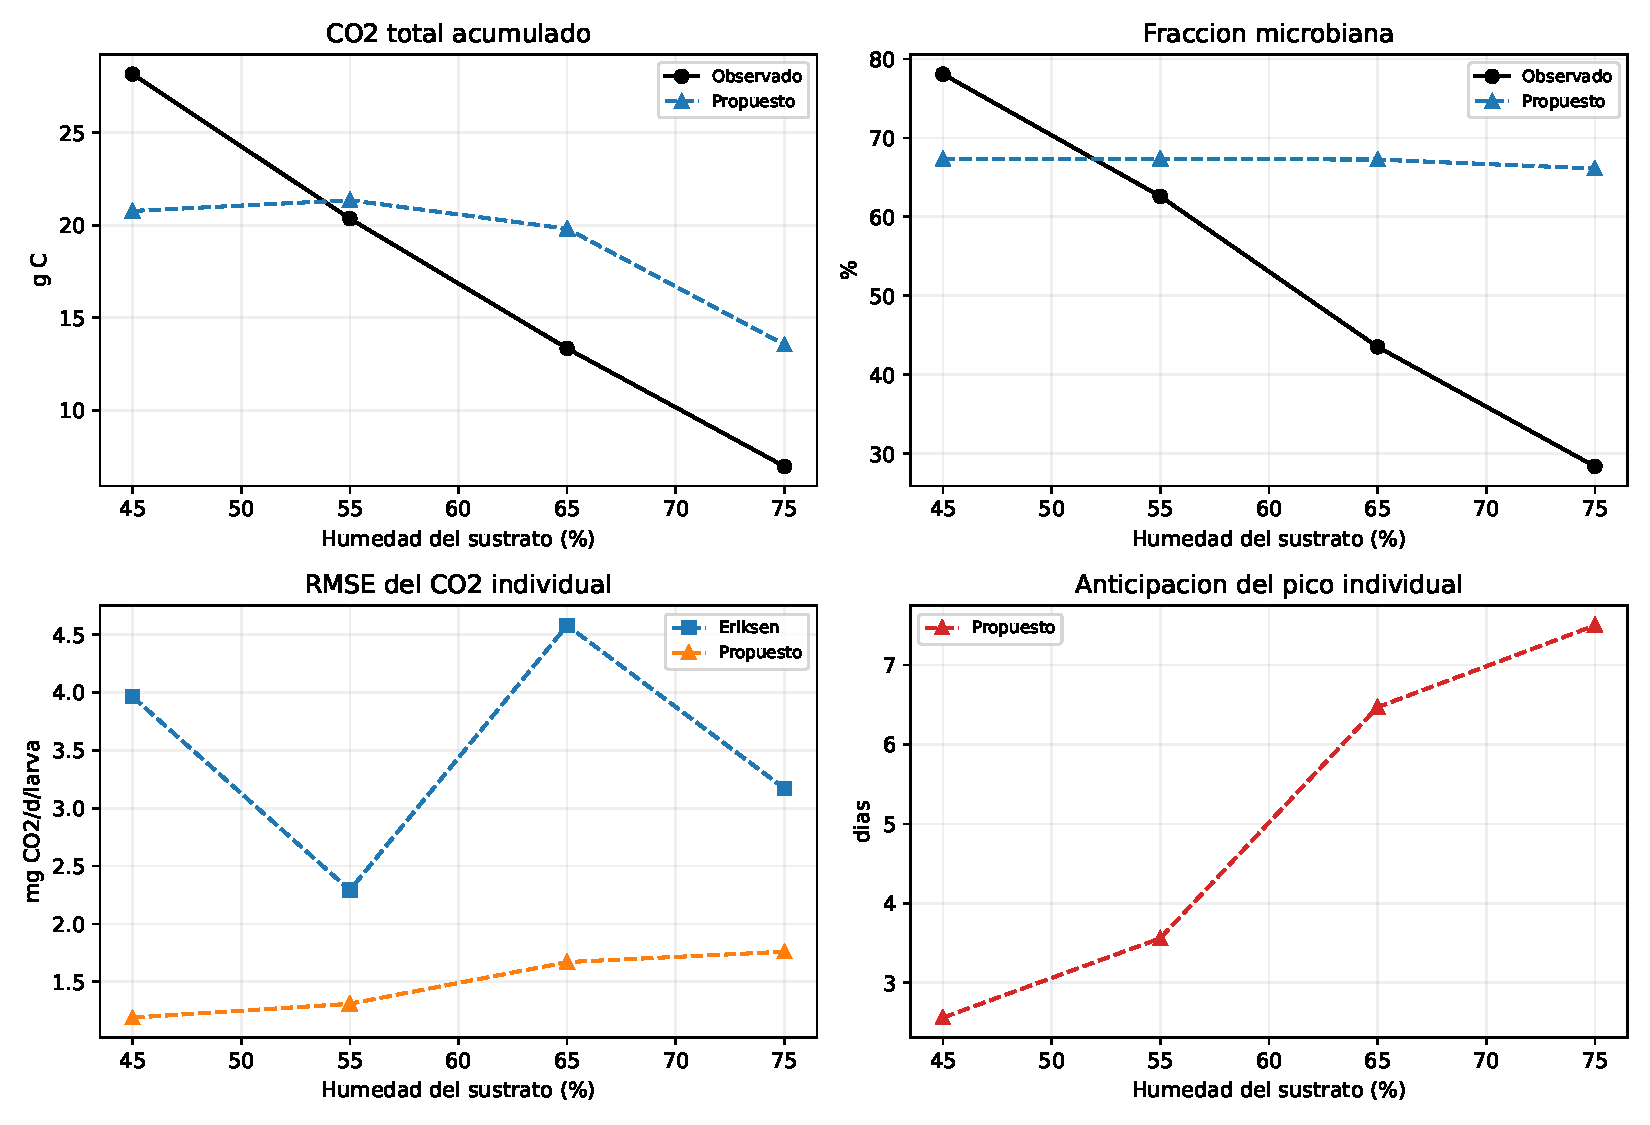
\includegraphics[width=\textwidth]{bekker_comparacion.pdf}
\caption{Evaluación detallada con Bekker: acumulado total, fracción
microbiana, error individual y anticipación del pico. La coincidencia
en algunos acumulados no implica una reproducción correcta de la
dinámica o de la partición entre fuentes.}
\label{fig:bekker}
\end{figure}

\subsection{Síntesis comparativa}

\begin{table}[H]
\centering
\small
\caption{Interpretación comparativa por estudio.}
\begin{tabularx}{\textwidth}{l X X}
\toprule
Estudio & Resultado favorable & Limitación principal \\
\midrule
Datos propios & Reduce el RMSE censurado $53{,}6$\,\% en calibración
y $31{,}95$\,\% en validación interna &
No mejora el RMSE exacto conjunto; el bootstrap exploratorio incluye
reducciones negativas \\
Laganaro & Eriksen reproduce el aumento de \co{} con baja calidad &
El propuesto no modifica $Y_B$ ni $m$ con la dieta \\
Bekker & El propuesto reduce el RMSE individual &
Anticipa picos y mantiene casi constante la fracción microbiana \\
Ermolaev & El propuesto reduce el RMSE de las tasas &
Sobrestima el acumulado y anticipa el pico \\
Schøn & Eriksen queda más cerca del rango observado &
El $Q_{10}$ propuesto impide representar el colapso térmico \\
Rossi & El propuesto reduce el RMSE neto agregado &
Ninguno reproduce las tres corridas ni el momento del pico \\
\bottomrule
\end{tabularx}
\end{table}
